\chapter{Arhitektura i dizajn sustava}
	
		\section{Baza podataka}
			
			\textbf{\textit{dio 1. revizije}}\\
			
		Za potrebe našeg sustava koristit ćemo relacijsku bazu podataka koja svojom strukturom olakšava modeliranje stvarnog svijeta. Gradivna jedinka baze je relacija, odnosno tablica koja je definirana svojim imenom i skupom atributa. Zadaća baze podataka je brza i jednostavna pohrana, izmjena i dohvat podataka za daljnju obradu. Baza podataka ove aplikacije sastoji se od sljedećih entiteta:
		\begin{packed_item}
			\item Korisnik
			\item Sudionik
			\item Animator
			\item Organizator
			\item Prijava
			\item Grupa
			\item Raspored
			\item Aktivnost
			\item Kamp
			\item ocjena\_aktivnosti
			\item ukupni\_dojam
		\end{packed_item}
			\subsection{Opis tablica}
			

				\textbf{Korisnik}	Ovaj entitet sadržava sve važne informacije o korisniku aplikacije. Sadrži atribute: korisnicko\_ime, lozinka, email, ime, prezime, status. Ovaj entitet u vezi je \textit{One-to-One} s entitetom Sudionik preko atributa korisnicko\_ime, u vezi \textit{One-to-One} s entitetom Animator preko atributa korisnicko\_ime, u vezi \textit{One-to-One} s entitetom Organizator preko atributa korisnicko\_ime, u vezi \textit{One-to-One} s entitetom Prijava preko atributa korisnicko\_ime, u vezi \textit{One-to-Many} s entitetom ocjena\_aktivnosti preko atributa korisnicko\_ime, te u vezi textit{One-to-One} s entitetom ukupni\_dojam preko atributa korisnicko\_ime.
				
				\begin{longtabu} to \textwidth {|X[6, l]|X[6, l]|X[20, l]|}
					
					\hline \multicolumn{3}{|c|}{\textbf{Korisnik }}	 \\[3pt] \hline
					\endfirsthead
					
					\hline \multicolumn{3}{|c|}{\textbf{Korisnik}}	 \\[3pt] \hline
					\endhead
					
					\hline 
					\endlastfoot
					
					\cellcolor{LightGreen}Korisnicko ime & VARCHAR	& jedinstveni identifikator korisnika\\ \hline
					Lozinka	& VARCHAR & lozinka korisnika	\\ \hline 
					Email & VARCHAR &  email korisnika \\ \hline 
					Ime & VARCHAR	&  ime korisnika		\\ \hline 
					Prezime & VARCHAR	& prezime korisnika 		\\ \hline 
					Status & VARCHAR	& status korisnika 		\\ \hline 
					
					
				\end{longtabu}
			
				\textbf{Sudionik}	Ovaj entitet sadržava sve važne informacije vezane za sudionika u kampu. Sadrži atribute: korisnicko\_ime\_sudionik, br\_tel\_sudionik, datum\_i\_god\_rod\_sudionik, br\_tel\_odg\_osobe, id\_grupa. Ovaj entitet je u vezi \textit{Many-to-one} s entitetom Grupa preko atributa id\_grupa, te u vezi \textit{One-to-One}  s entitetom Korisnik preko atributa korisnicko\_ime\_sudionik.
				
				\begin{longtabu} to \textwidth {|X[6, l]|X[6, l]|X[20, l]|}
					
					\hline \multicolumn{3}{|c|}{\textbf{Sudionik}}	 \\[3pt] \hline
					\endfirsthead
					
					\hline \multicolumn{3}{|c|}{\textbf{Sudionik}}	 \\[3pt] \hline
					\endhead
					
					\hline 
					\endlastfoot
					
					\cellcolor{LightGreen}Korisnicko ime sudionik & VARCHAR	&  jedinstveni identifikator korisnika( sudionika) 	\\ \hline
					Br tel sudionik	& INT & broj telefona sudionika   	\\ \hline 
					Datum i god rod sudionik & DATE & datum i godina rođenja sudionika  \\ \hline 
					Br tel odg osobe & INT	&  broj telefona odgovorne osobe( ako je sudionik mlađi od 18)		\\ \hline
					\cellcolor{LightBlue} ID grupa	& INT & jedinstveni identifikator grupe sudionika  	\\ \hline 
					
					
				\end{longtabu}
			
				\textbf{Animator}	Ovaj entitet sadržava sve važne informacije vezane za animatora u kampu. Sadrži atribute: korisnicko\_ime\_animator, br\_tel\_animator, datum\_i\_god\_rod\_animator. Ovaj entitet je u \textit{One-to-One} vezi s entitetom Korisnik preko atributa korisnicko\_ime\_animatora, te u vezi \textit{Many-to-One} s entitetom Raspored preko atributa korisnicko\_ime\_animator.
				
				\begin{longtabu} to \textwidth {|X[6, l]|X[6, l]|X[20, l]|}
					
					\hline \multicolumn{3}{|c|}{\textbf{Animator}}	 \\[3pt] \hline
					\endfirsthead
					
					\hline \multicolumn{3}{|c|}{\textbf{Animator}}	 \\[3pt] \hline
					\endhead
					
					\hline 
					\endlastfoot
					
					\cellcolor{LightGreen}Korisnicko ime animator & VARCHAR	&  jedinstveni identifikator korisnika( animatora)	\\ \hline
					Br tel animator	& INT &  broj telefona animatora 	\\ \hline 
					Datum i god rod animator & DATE & datum i godina rođenja animatora   \\ \hline 
					
					
				\end{longtabu}
			
				\textbf{Organizator}	Ovaj entitet sadrži sve važne informacije vezane za organizatora kampa. Sadrži atribut: korisnicko\_ime\_organizator. Ovaj entitet je u \textit{One-to-One} vezi s entitetom Korisnik preko atributa korisnicko\_ime\_organizator.
				
				\begin{longtabu} to \textwidth {|X[6, l]|X[6, l]|X[20, l]|}
					
					\hline \multicolumn{3}{|c|}{\textbf{Organizator}}	 \\[3pt] \hline
					\endfirsthead
					
					\hline \multicolumn{3}{|c|}{\textbf{Organizator}}	 \\[3pt] \hline
					\endhead
					
					\hline 
					\endlastfoot
					
					\cellcolor{LightGreen}Korisnicko ime organizator & VARCHAR	& jedinstveni identifikator korisnika( organizatora)	\\ \hline
				
					
					
				\end{longtabu}
			
				\textbf{Prijava}	Ovaj entitet sadrži sve važne informacije vezane o prijavama na kamp. Sadrži atribute: id\_prijava, korisnicko\_ime, datum\_i\_vrijeme\_prijave, status\_prijava, ime\_kamp, motivacijsko\_pismo, datum\_odrzavanja\_kamp. Ovaj entitet je u \textit{One-to-One} vezi s entitetom Korisnik preko atributa korisnicko\_ime, te u \textit{Many-to-One} vezi s entitetom Kamp preko atributa ime\_kamp.
				
				\begin{longtabu} to \textwidth {|X[6, l]|X[6, l]|X[20, l]|}
					
					\hline \multicolumn{3}{|c|}{\textbf{Prijava}}	 \\[3pt] \hline
					\endfirsthead
					
					\hline \multicolumn{3}{|c|}{\textbf{Prijava}}	 \\[3pt] \hline
					\endhead
					
					\hline 
					\endlastfoot
					
					\cellcolor{LightGreen}ID prijava & INT	& jedinstveni identifikator prijave  	\\ \hline
					\cellcolor{LightBlue}Korisnicko ime	& VARCHAR & jedinstveni identifikator korisnika  	\\ \hline 
					Datum i vrijeme prijava & DATETIME &  datum i vrijeme prijave \\ \hline 
					Status prijava & BOOLEAN	&  status prijave		\\ \hline 
					\cellcolor{LightBlue}Ime kamp	& VARCHAR &  ime kampa 	\\ \hline
					Motivacijsko pismo & VARCHAR	&  motivacijsko pismo prijave	\\ \hline 
					Datum odrzavanja kamp & DATE	& datum održavanja kampa	\\ \hline 
					
					
				\end{longtabu}
			
				\textbf{Grupa}	Ovaj entitet sadrži sve važne informacije o grupama na kampu. Sadrži atribute: id\_grupa, ime\_grupa. Ovaj entitet je u \textit{One-to-Many} vezi s entitetom Sudionik preko atributa id\_grupa, te u vezi \textit{Many-to-One} s entitetom Raspored preko atributa id\_grupa.
				
				\begin{longtabu} to \textwidth {|X[6, l]|X[6, l]|X[20, l]|}
					
					\hline \multicolumn{3}{|c|}{\textbf{Grupa}}	 \\[3pt] \hline
					\endfirsthead
					
					\hline \multicolumn{3}{|c|}{\textbf{Grupa}}	 \\[3pt] \hline
					\endhead
					
					\hline 
					\endlastfoot
					
					\cellcolor{LightGreen}ID grupa & INT	& jedinstveni identifikator grupe 		\\ \hline
					Ime grupa	& VARCHAR & ime grupe   	\\ \hline 
					
				\end{longtabu}
			
				\textbf{Raspored}	Ovaj entitet sadrži sve važne informacije vezane za raspored kampa. Sadrži atribute: id\_grupa, id\_aktivnost, datum\_i\_vrijeme\_izvrsavanja, korisnicko\_ime\_animator. Ovaj entitet je u \textit{One-to-Many} vezi s entitetom Grupa preko atributa id\_grupa, \textit{Many-to-Many} vezi s entitetom Animator preko atributa korisnicko\_ime\_animator, te u vezi \textit{One-to-Many} s entitetom Aktivnost preko atributa id\_aktivnost.
				
				\begin{longtabu} to \textwidth {|X[6, l]|X[6, l]|X[20, l]|}
					
					\hline \multicolumn{3}{|c|}{\textbf{Raspored}}	 \\[3pt] \hline
					\endfirsthead
					
					\hline \multicolumn{3}{|c|}{\textbf{Raspored}}	 \\[3pt] \hline
					\endhead
					
					\hline 
					\endlastfoot
					
					\cellcolor{LightGreen}ID grupa & INT	&  jedinstveni identifikator grupe	\\ \hline
					\cellcolor{LightGreen}ID aktivnost	& INT & jedinstveni identifikator aktivnosti  	\\ \hline 
					\cellcolor{LightGreen}Datum i vrijeme izvrsavanja & DATETIME & datum i vrijeme izvršavanja    \\ \hline 
					\cellcolor{LightBlue}Korisnicko ime animator & VARCHAR	&  jedinstveni identifikator korisnika( animator)	\\ \hline 
					
					
					
				\end{longtabu}
			
			
				\textbf{Aktivnost}	Ovaj entitet sadrži sve važne o informacijama vezane za aktivnosti na kampu. Sadrži atribute: id\_aktivnost, ime\_aktivnost, opis\_aktivnost, trajanje\_aktivnost\_(sat/i), tip\_aktivnosti, datum\_odrzavanja\_kamp, ime\_kamp. Ovaj entitet je u \textit{One-to-Many} vezi s entitetom ocjena\_aktivnosti preko atributa id\_aktivnost, u \textit{Many-to-Many} vezi s entitetom Kamp preko atributa ime\_kamp, te u \textit{Many-to-One} vezi s entitetom Raspored preko atributa id\_aktivnost.
				
				\begin{longtabu} to \textwidth {|X[6, l]|X[6, l]|X[20, l]|}
					
					\hline \multicolumn{3}{|c|}{\textbf{Aktivnost}}	 \\[3pt] \hline
					\endfirsthead
					
					\hline \multicolumn{3}{|c|}{\textbf{Aktivnost}}	 \\[3pt] \hline
					\endhead
					
					\hline 
					\endlastfoot
					
					\cellcolor{LightGreen}ID aktivnost & INT	& jedinstveni identifikator aktivnosti  	\\ \hline
					Ime aktivnost	& VARCHAR &  ime aktivnosti 	\\ \hline 
					Opis aktivnost & VARCHAR & opis aktivnosti  \\ \hline 
					Trajanje aktivnost (sat/i) & DECIMAL	& trajanje aktivnosti 		\\ \hline
					Tip aktivnost & VARCHAR	& tip aktivnosti  		\\ \hline 
					Datum odrzavanja kamp & DATE	&  datum održavanja kampa		\\ \hline 
					\cellcolor{LightBlue} Ime kamp	& VARCHAR &  ime kampa 	\\ \hline 
					
					
				\end{longtabu}
			
				\textbf{Kamp}	Ovaj entitet sadrži sve važne informacije o kampu. Sadrži atribute: ime\_kamp, datum\_odrzavanja\_kamp, trajanje\_(dan/a), pocetak\_prijava\_sudionika, kraj\_prijava\_sudionika, pocetak\_prijava\_animatora, kraj\_prijava\_animatora, broj\_grupa, status, email\_kamp. Ovaj entitet je u \textit{Many-to-Many} vezi s entitetom Aktivnost preko atributa ime\_kamp, u \textit{One-to-Many} vezi s entitetom Prijava preko atributa ime\_kamp, te u \textit{One-to-Many} vezi s entitetom ukupni\_dojam preko atributa ime\_kamp i datum\_odrzavanja\_kamp.
				
				\begin{longtabu} to \textwidth {|X[6, l]|X[6, l]|X[20, l]|}
					
					\hline \multicolumn{3}{|c|}{\textbf{Kamp}}	 \\[3pt] \hline
					\endfirsthead
					
					\hline \multicolumn{3}{|c|}{\textbf{Kamp}}	 \\[3pt] \hline
					\endhead
					
					\hline 
					\endlastfoot
					
					\cellcolor{LightGreen}Ime kamp & VARCHAR	&  ime kampa	\\ \hline
					\cellcolor{LightGreen}Datum odrzavanja kamp & DATE	& datum održavanja kampa 	\\ \hline
					Trajanje (dan/a)	& INT & trajanje kampa  	\\ \hline 
					Pocetak prijava sudionika & DATETIME & datum i vrijeme početka prijave sudionika  \\ \hline 
					Kraj prijava sudionika& DATETIME	& datum i vrijeme  kraja prijave sudionika	\\ \hline 
					Pocetak prijava animatora& DATETIME	& datum i vrijeme pocetka prijava animatora 		\\ \hline 
					Kraj prijava animatora & DATETIME& datum i vrijeme kraja prijava animatora 		\\ \hline 
					Broj grupa & INT	& broj grupa 		\\ \hline 
					Status & VARCHAR	& status kampa 		\\ \hline
					Email kamp & VARCHAR	& email adresa kampa 		\\ \hline
					
					
				\end{longtabu}
			
				\textbf{ocjena\_aktivnosti}	Ovaj entitet sadrži sve važne informacije o ocjenama aktivnosti. Sadrži atribute: korisnicko\_ime, ocjena, dojam, id\_aktivnost. Ovaj entitet je u \textit{Many-to-one} vezi s entitetom Korisnik preko atributa korisnicko\_ime, te u \textit{Many-to-One} vezi s entitetom Aktivnost preko atributa id\_aktivnost.   
				
				\begin{longtabu} to \textwidth {|X[6, l]|X[6, l]|X[20, l]|}
					
					\hline \multicolumn{3}{|c|}{\textbf{ocjena\_aktivnosti}}	 \\[3pt] \hline
					\endfirsthead
					
					\hline \multicolumn{3}{|c|}{\textbf{ocjena\_aktivnosti}}	 \\[3pt] \hline
					\endhead
					
					\hline 
					\endlastfoot
					
					\cellcolor{LightGreen}Korisnicko ime& VARCHAR	& jedinstveni identifikator korisnika	\\ \hline
					Ocjena	& INT & ocjena aktivnosti  	\\ \hline 
					Dojam  & VARCHAR &  dojam aktivnosti   \\ \hline 
					\cellcolor{LightGreen}ID aktivnost	& INT & jedinstveni identifikator aktivnosti	\\ \hline 
					
					
				\end{longtabu}
			
				\textbf{ukupni\_dojam}	Ovaj entitet sadrži sve važne informacije o ukupnom dojmu o aktivnosti. Sadrži atribute: korisnicko\_ime, ocjena, dojam, ime\_kamp, datum\_odrzavanja\_kamp. Ovaj entitet je u \textit{Many-to-One} vezi s entitetom Kamp preko atributa ime\_kamp i atributa datum\_odrzavanja\_kamp, te u \textit{One-to-One} vezi s entitetom Korisnik preko atributa korisnicko\_ime.
				
				\begin{longtabu} to \textwidth {|X[6, l]|X[6, l]|X[20, l]|}
					
					\hline \multicolumn{3}{|c|}{\textbf{ukupni\_dojam}}	 \\[3pt] \hline
					\endfirsthead
					
					\hline \multicolumn{3}{|c|}{\textbf{ukupni\_dojam}}	 \\[3pt] \hline
					\endhead
					
					\hline 
					\endlastfoot
					
					\cellcolor{LightGreen}Korisnicko ime sudionik & VARCHAR	& korisnicko ime korisnika( sudionik) 	\\ \hline
					\cellcolor{LightGreen}Datum odrzavanja kampa	& DATE & datum odrzavanja kampa  	\\ \hline 
					Dojam & VARCHAR & dojam ukupnog iskustva  \\ \hline 
					\cellcolor{LightBlue} Ime kamp	& VARCHAR & ime kampa  	\\ \hline 
					Ocjena & INT & ocjena  ukupnog iskustva 	\\ \hline 
					
					
				\end{longtabu}
			
			\eject
			
			
			\subsection{Dijagram baze podataka}
				\begin{figure}[H]
				\centerline{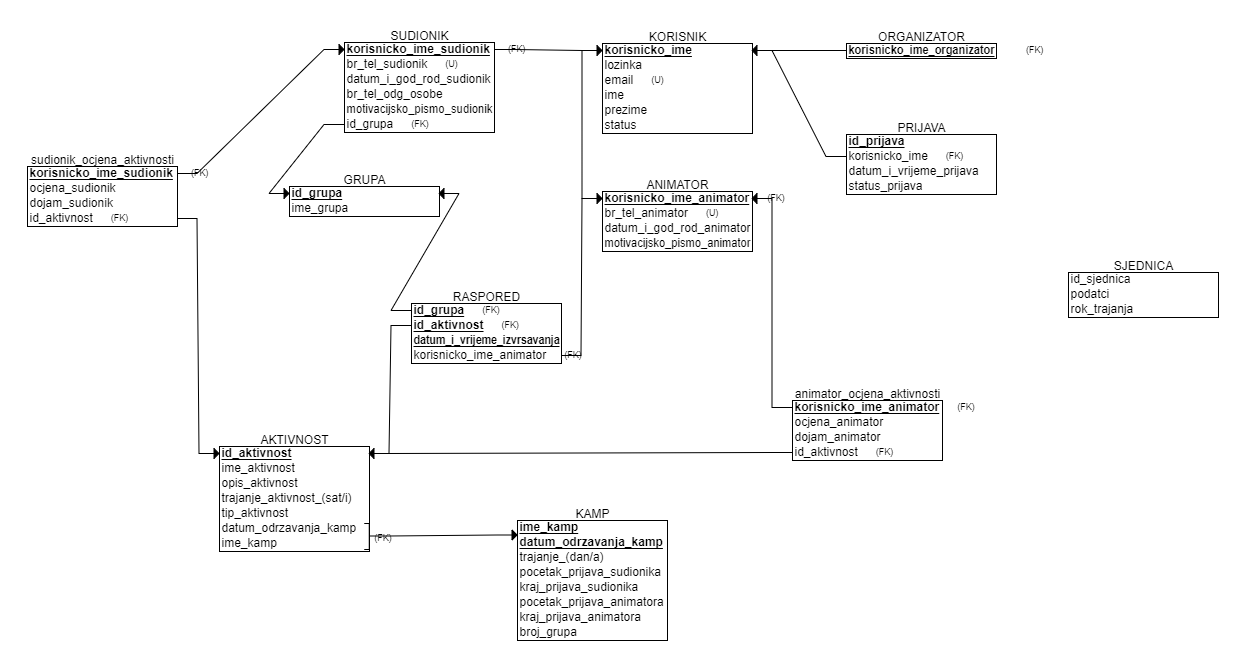
\includegraphics[width=\linewidth]{slike/ER_model_baze.png}}
				\caption{E-R dijagram baze podataka}
				\label{fig:ERdijagram}
			\end{figure}
			
			\eject
			
			
		\section{Dijagram razreda}
		
		U ovom poglavlju nalazi se dijagram razreda sa svim potrebnim klasama za rad sustava. Na slici 4.2 je prikazan dijagram razreda. On preslikava strukturu baze podataka u aplikaciji. Implementirane metode direktno komuniciraju s bazom podataka te vraćaju tražene podatke. Razred Korisnik predstavlja općenitog korisnika sustava, kojeg nasljeđuju razredi Sudionik, Organizator i Animator, koji predstavljaju sudionika na kampu, organizatora, odnosno voditelja kampa te animatore na kampu.
			\begin{figure}[H]
				\centerline{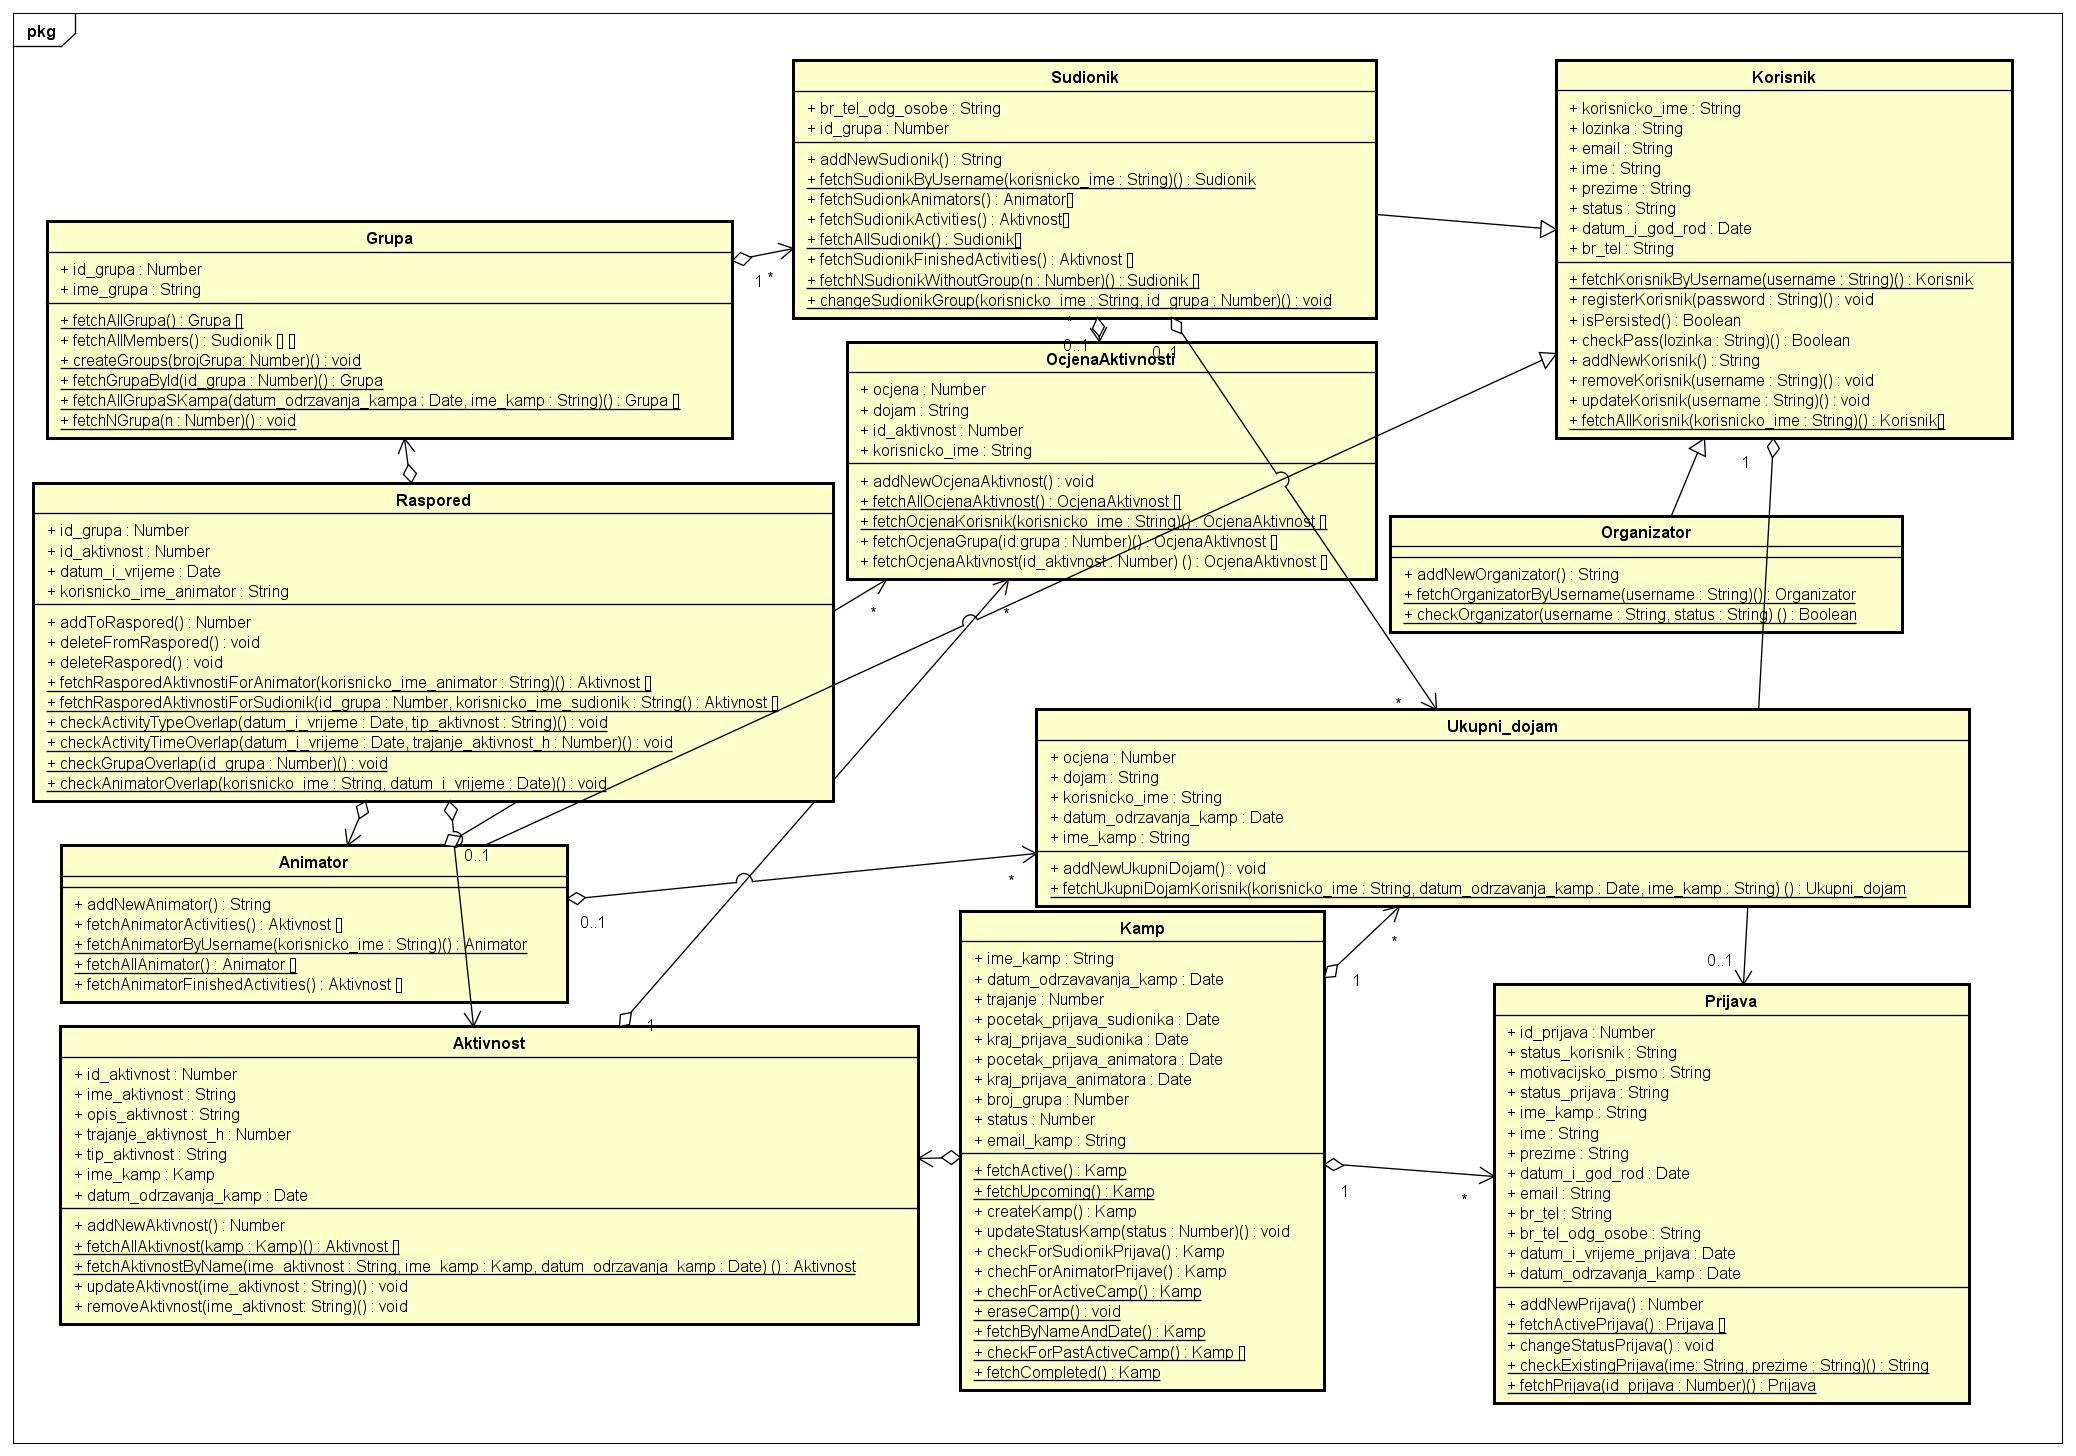
\includegraphics[width=\linewidth]{slike/Dijagram_razreda_modeli.png}}
				\caption{Dijagram razreda- modeli}
				\label{fig:dijagram_razreda_modeli}
			\end{figure}
			
			\eject
		
		\section{Dijagram stanja}
		
		Dijagram stanja prikazuje stanje objekta te prijelaze iz jednog stanja u drugo temeljene na događajima. Na slici 4.3 je prikazan dijagram stanja za registriranog sudionika. Nakon prijave, sudioniku se prikazuje početna stranica na kojoj se prikazuju sudionikov raspored te popis aktivnosti na kojima je sudjelovao. Sudionik može ocijeniti aktivnosti na kojima je sudjelovao, te po završetku kampa može ostaviti ukupni dojam. Također, sudionik može u izborniku odabrati neku od ponuđenih mogućnosti. Klikom na "Moj profil" prikazuju mu se njegovi osobni podatci. Klikom na "Moja grupa" prikazuju mu se podaci njegove grupe. Na slici 4.4 je prikazan dijagram stanja za organizatora. Nakon prijave, organizator na početnoj stranici može otvoriti izbornik te odabrati neku od ponuđenih mogućnosti. Klikom na "Stvori novi kamp" organizator može stvoriti novi kamp. Klikom na "Stvori novu aktivnost" organizator može stvoriti novu aktivnost. Klikom na "Prijave za kamp" organizator obrađuje pristigle prijave za kamp. Klikom na "Stvori Grupe" organizator može pregledati i stvoriti nove grupe te premjestiti sudionike. Klikom na "Moj profil" organizatoru se prikazuju njegovi osobni podatci.  
		\begin{figure}[H]
			\centerline{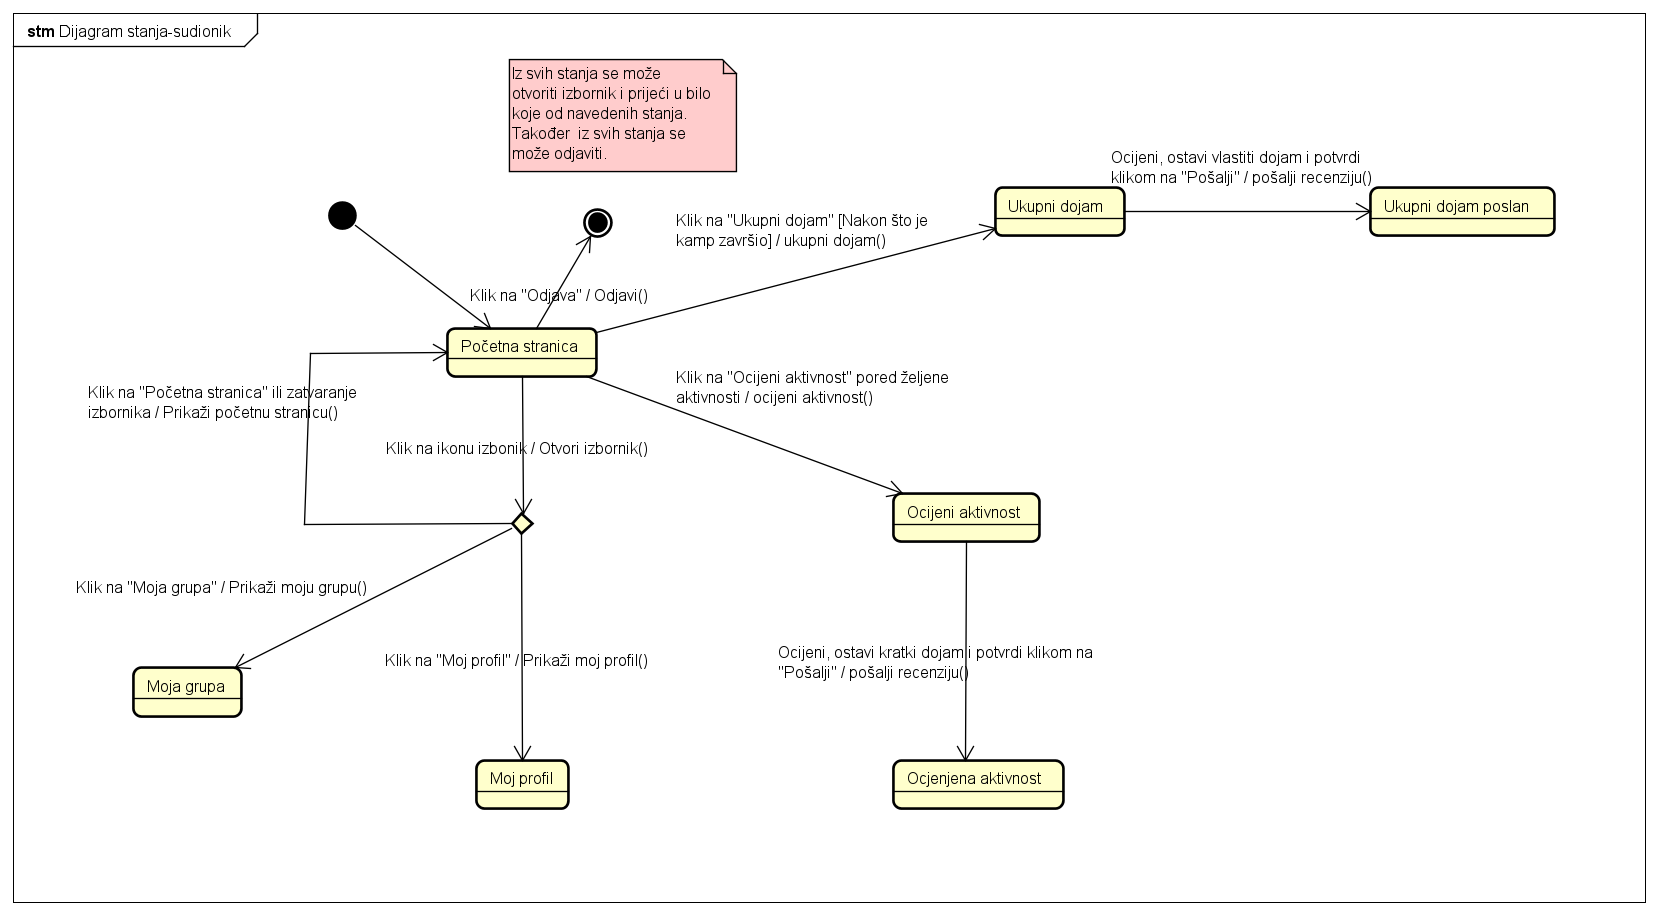
\includegraphics[width=\linewidth]{slike/Dijagram_stanja_sudionik.png}}
			\caption{Dijagram stanja- sudionik }
			\label{fig:dijagram_stanja_sudionik}
		\end{figure}
		
		\eject	
		
		\begin{figure}[H]
			\centerline{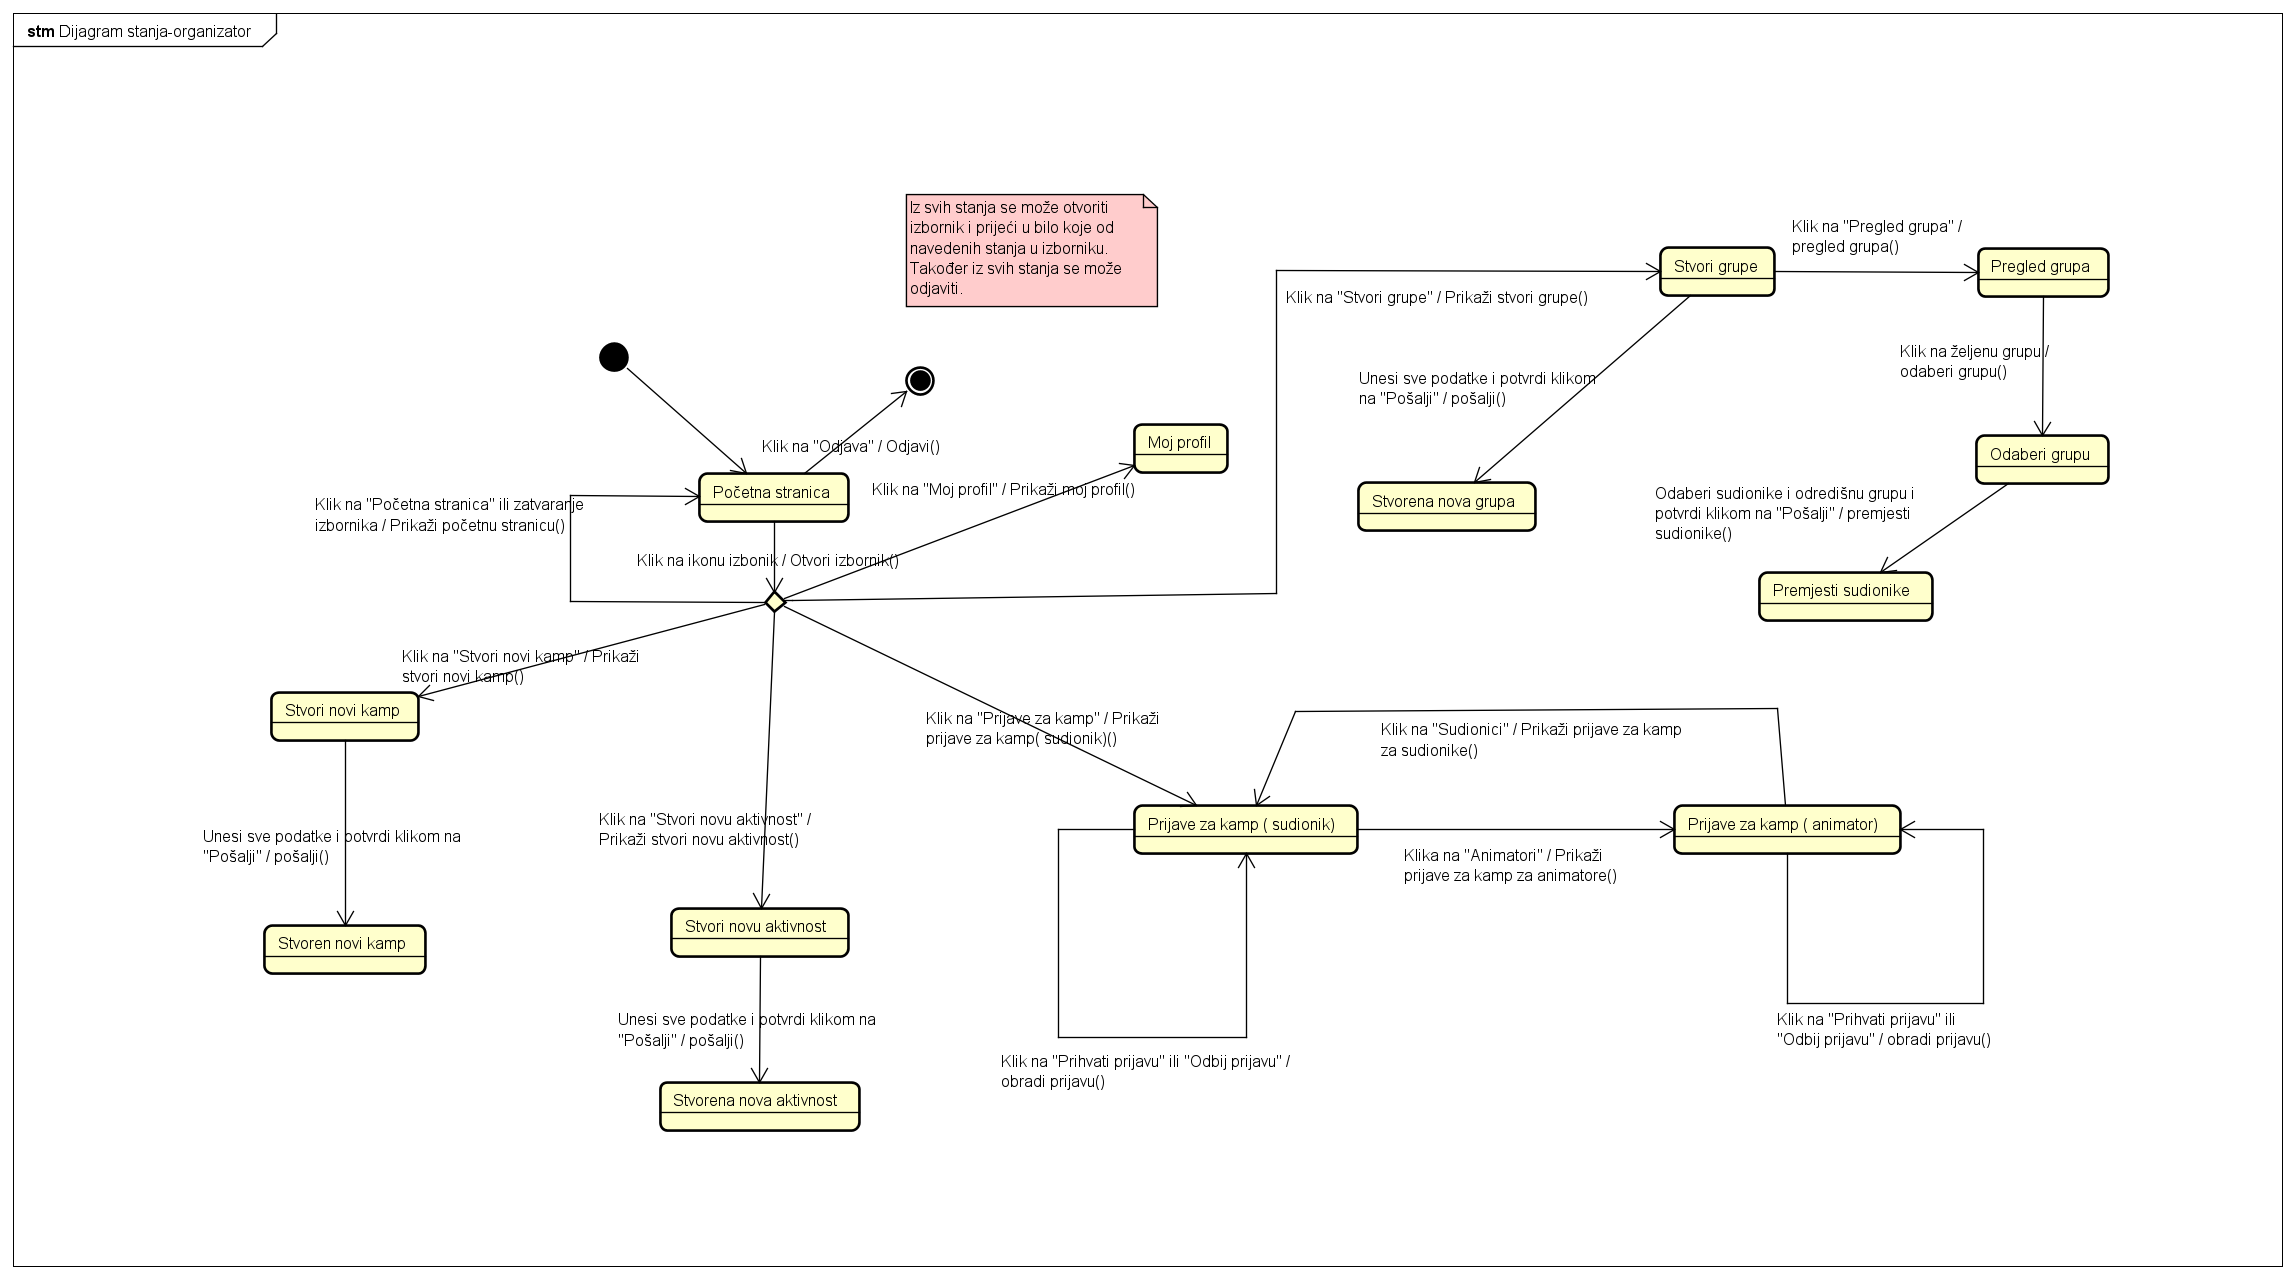
\includegraphics[width=\linewidth]{slike/Dijagram_stanja_organizator.png}}
			\caption{Dijagram stanja- organizator }
			\label{fig:dijagram_stanja_organizator}
		\end{figure}
		
		\eject	
		
		\section{Dijagram aktivnosti}
		
		Dijagram aktivnosti primjenjuje se za opis modela toka upravljanja ili toka podataka. Ne upotrebljava se za modeliranje događajima poticanog ponašanja. U modeliranju toka upravljanja svaki novi korak poduzima se nakon završenog prethodnog. Na dijagramu aktivnosti 4.5 prikazan je postupak premještanja sudionika u drugu grupu, sa strane organizatora. Korisnik se prijavljuje u sustav, otvara izbornik, otvara stranicu za stvaranje grupa, pregledava grupe, odabire željene sudionike i odredišnu grupu, što se zatim pohranjuje u sustav.
			\begin{figure}[H]
			\centerline{\includegraphics[width=\linewidth]{slike/Dijagram aktivnosti-premještanje sudionika.png}}
			\caption{Dijagram aktivnosti-premještanje sudionika}
			\label{fig:dijagram_aktivnosti}
		\end{figure}
		
		\eject		

		
	